\documentclass{beamer}

\usepackage[frenchb]{babel}
\usepackage[T1]{fontenc}
\usepackage[utf8]{inputenc}
\usepackage{textcomp}

\usetheme{PaloAlto}

\title{Reconnaissance de musique fredonnée}
\author{F. Ecochard \and A. Grillet}
\institute{ENSEIRB-Mmk, Département électronique}
\date{\today}

\AtBeginSection[]
{
	\begin{frame}
		\frametitle{Sommaire}
		\tableofcontents[currentsection, hideothersubsections]
	\end{frame} 
}

\begin{document}
	\logo{
\includegraphics[height=10mm]{Enseirb_inp_logo.png}}
	\begin{frame}
		\titlepage
	\end{frame}
	\begin{frame}
		\frametitle{Table des matières}
		\tableofcontents
	\end{frame}

\section{Introduction}
	\begin{frame}
		\frametitle{Définition du sujet}
		\begin{alertblock}{Problème} % Bloc alerte rouge
			Musique dans la tête, sans connaître les paroles
		\end{alertblock}
		\begin{exampleblock}{Solution} % Bloc alerte rouge
			Reconnaissance de la musique fredonnée
		\end{exampleblock}
		\textbf{Article utilisé :} \\
		\textit{Query By Humming} : Musical Information Retrieval In An Audio Database
	\end{frame}
	\begin{frame}
		\frametitle{Organisation}
		\textbf{Outils : }Trello, Github
		
		\textbf{Timetable :}
		\begin{center}
			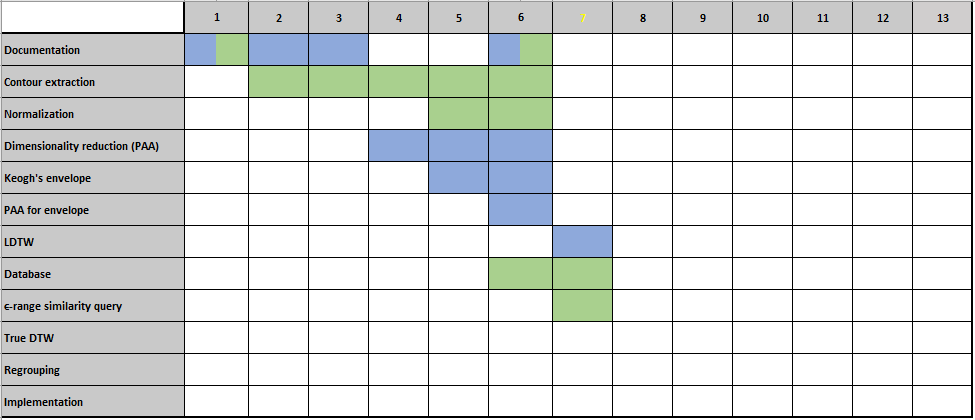
\includegraphics[width=10cm]{orga.PNG}
		\end{center}
		\colorbox[HTML]{A9D08E}{\textcolor[HTML]{FFFFFF}{Florent}}
		\colorbox[HTML]{8ea9db}{\textcolor[HTML]{FFFFFF}{Arnaud}}
	\end{frame}
	\begin{frame}
		\frametitle{Première séance}
		\begin{itemize}
			\item Documentation
			\item Recherche
			\item Mise en place de l'organisation
		\end{itemize}
	\end{frame}

\section{Détection du contour}
	\subsection{Première approche}
		\begin{frame}
			\frametitle{Méthode temporelle}
			Zero-crossing : Détection des \textit{passages à 0} \textrightarrow  période
			\begin{alertblock}{Problème} % Bloc alerte rouge
				Plusieurs PàZ par période :
			\end{alertblock}
			\centering 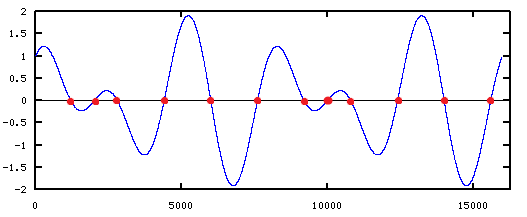
\includegraphics[width=8cm]{zero_crossing.PNG}
			
			Solution : Approche fréquentielle, auto-corrélation.
		\end{frame}
	\subsection{Auto-corrélation}
		\begin{frame}
			\frametitle{Méthode par auto-corrélation}
			Par fenêtre :
			\begin{itemize}
				\item Normalisation
				\item Seuillage fréquentiel
				\item Recherche premier maximum
				\item Comparaison seuil amplitude
			\end{itemize}
			\centering 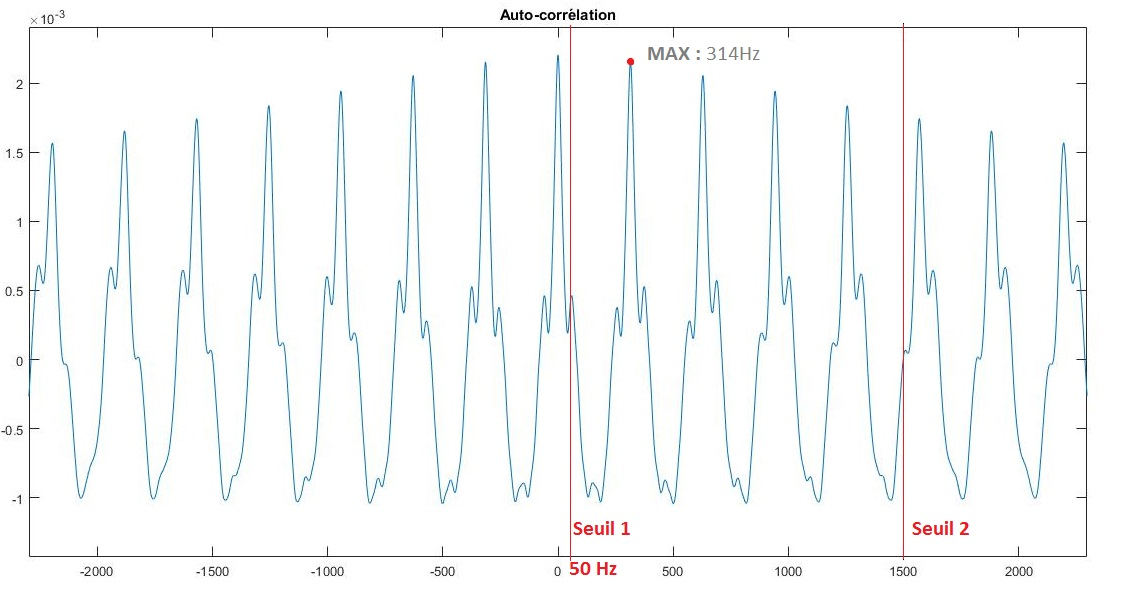
\includegraphics[width=8cm]{autocor.jpg}
		\end{frame}
	\subsection{Résultat}
		\begin{frame}
			\frametitle{Résultat pour une mélodie chantée}
			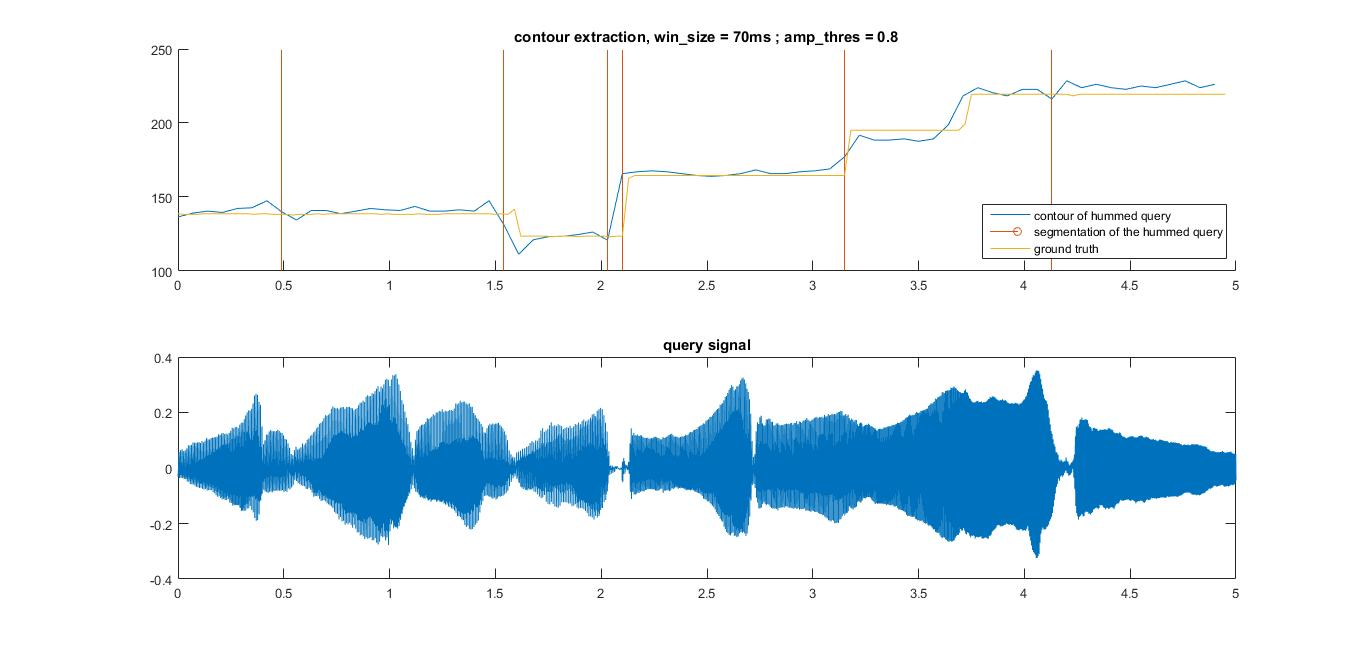
\includegraphics[width=11cm]{contour_result.jpg}
		\end{frame}
		\begin{frame}
			\frametitle{Résultat pour une mélodie fredonnée}
			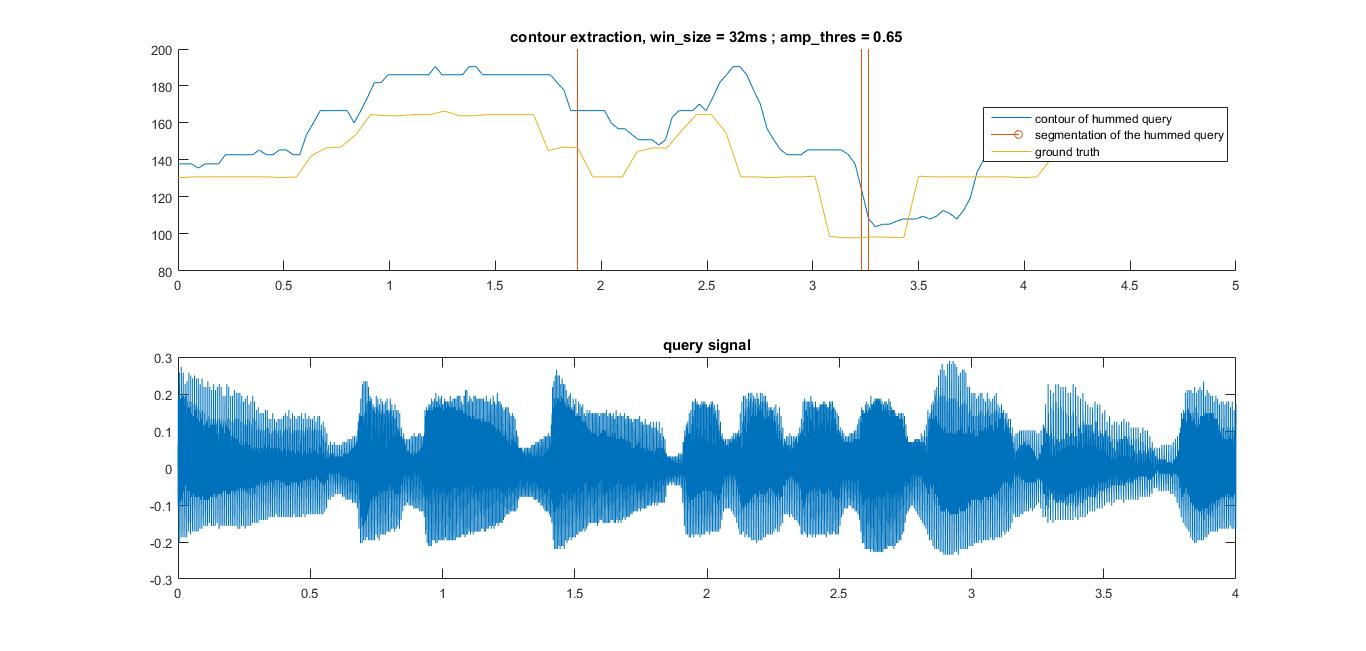
\includegraphics[width=11cm]{contour_result_hummed.jpg}
			
			\textrightarrow Problèmes : hauteur générale/locale, rythme global/local
		\end{frame}
\subsection{Normalisation}
	\begin{frame}
		\frametitle{Contour de la mélodie fredonnée après normalisation}
		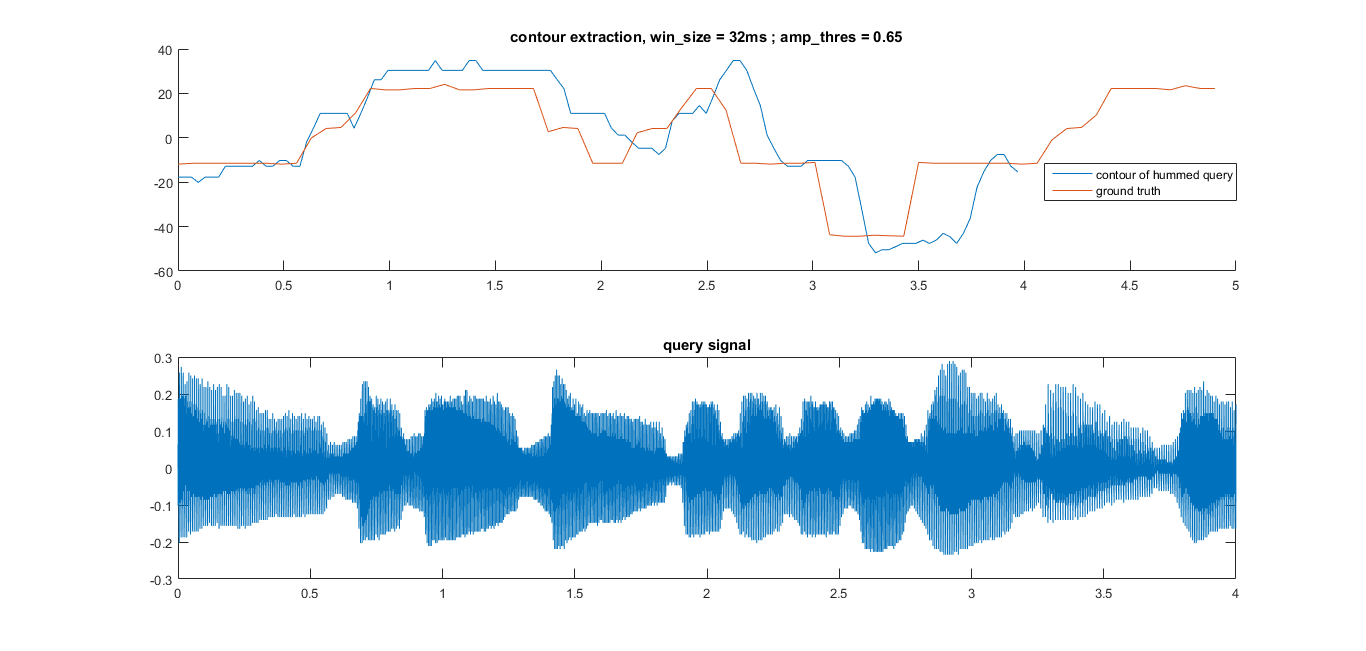
\includegraphics[width=11cm]{contour_norm.png}
		
		\textrightarrow Problèmes : hauteur locale, rythme global/local
	\end{frame}
\section{PAA}
\begin{frame}
	\frametitle{PAA (Piecewise Aggregate Function)}
	\begin{exampleblock}{but}
		Réduire la taille des vecteurs
		
	\end{exampleblock}
	\begin{equation}
		\overline{x_i}=\frac{M}{n}\times \sum_{j=\frac{n}{M}(i-1)+1}^{\frac{n}{M}+i}x_j
	\end{equation}
\end{frame}
\begin{frame}
	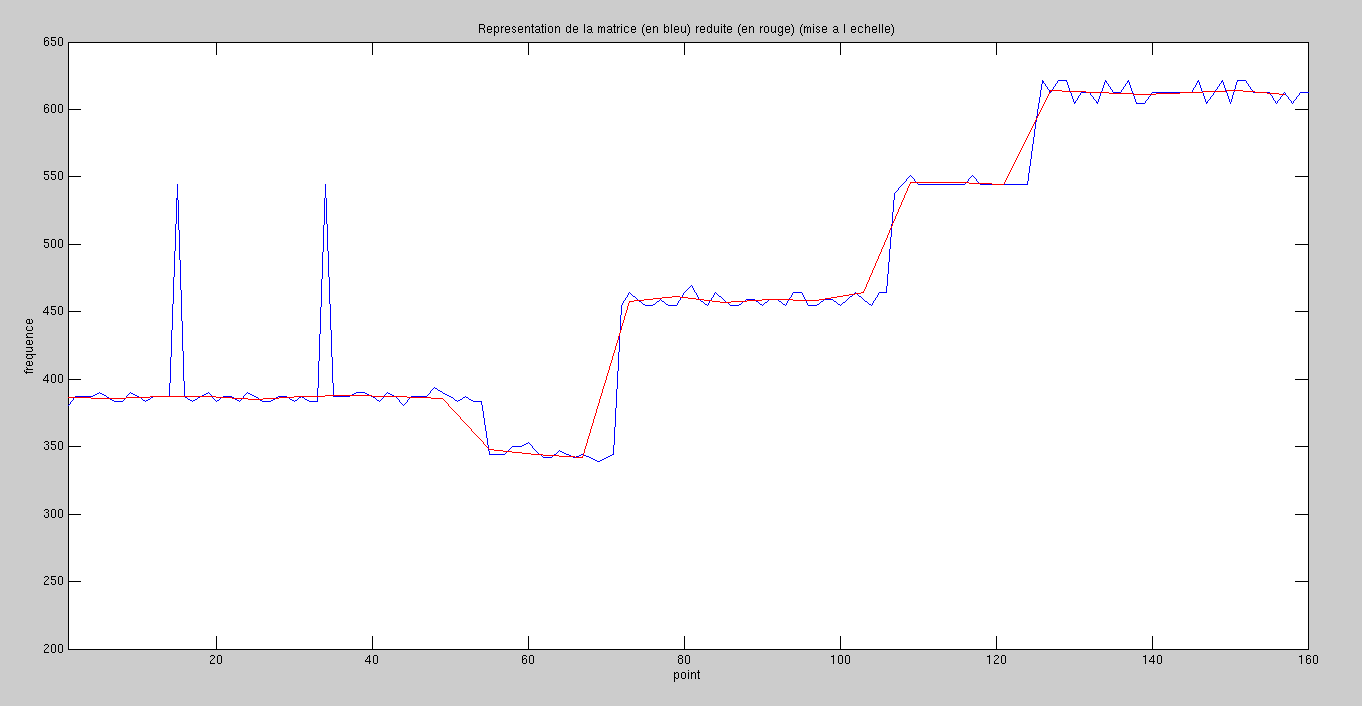
\includegraphics[width=10cm]{Representation_Matrice.png}
\end{frame}
\section{Enveloppe}
\begin{frame}
	\frametitle{Tracer l'enveloppe}
	\framesubtitle{Trouver valeurs max et min de l'enveloppe}
	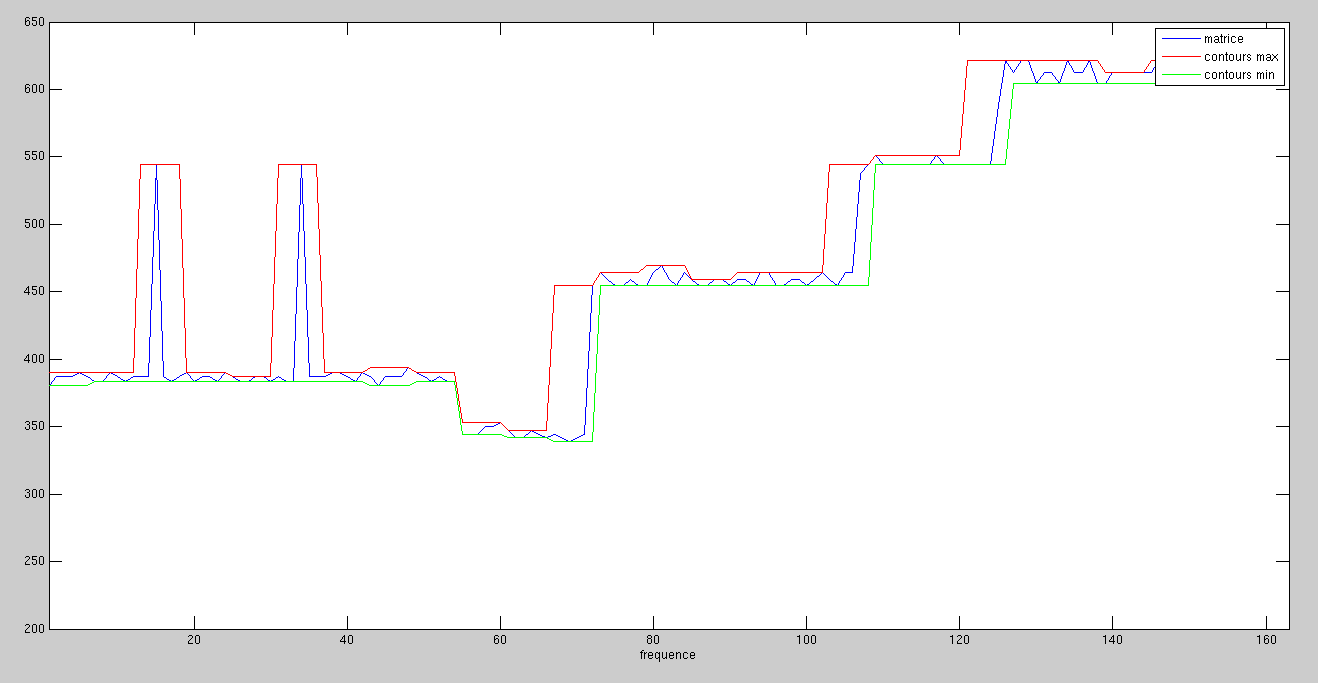
\includegraphics[width=11cm]{Contours_matrice.png}
\end{frame}
\begin{frame}
	\frametitle{Réduction taille enveloppe}
	\framesubtitle{Trouver valeurs max et min de l'enveloppe}
	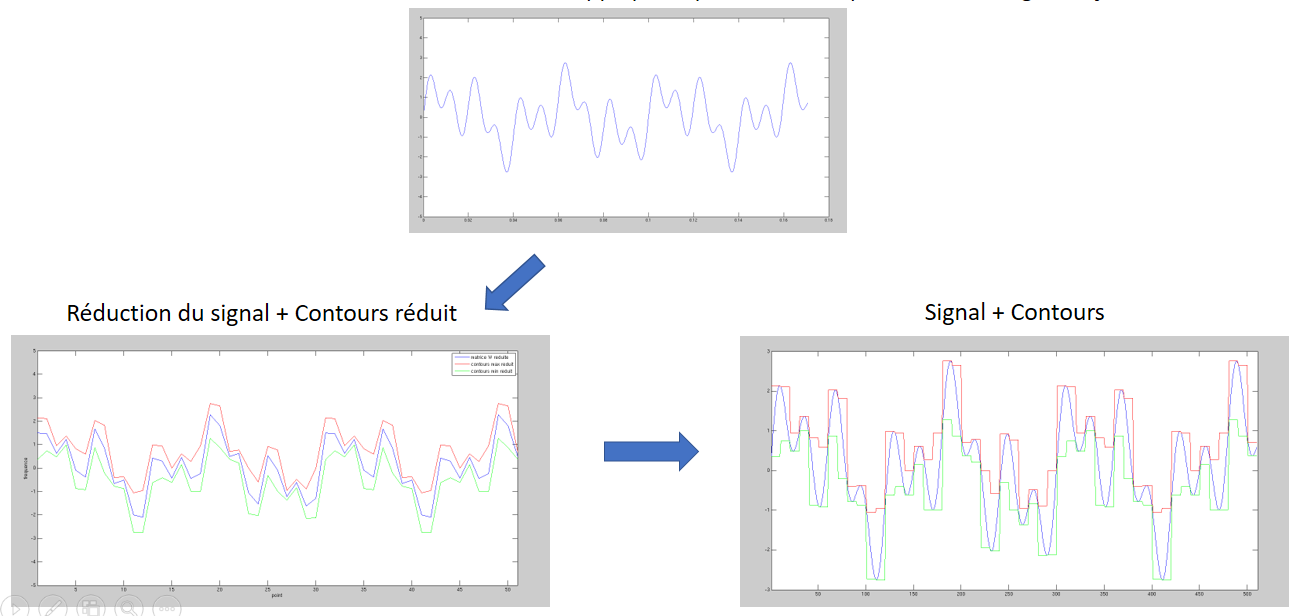
\includegraphics[width=11cm]{enveloppe.PNG}
\end{frame}
\begin{frame}
	\frametitle{Simulation Finale}
	\framesubtitle{Vecteur réduit avec enveloppes réduites}
	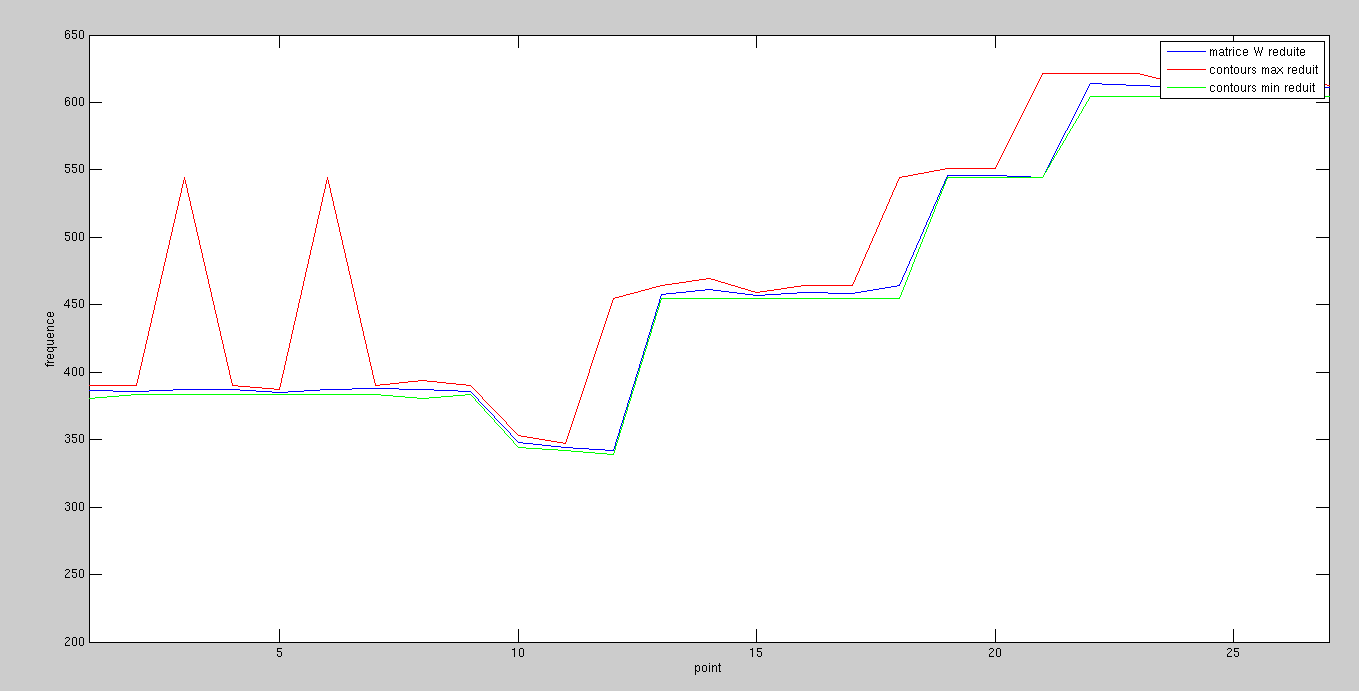
\includegraphics[width=10cm]{Contour_matrice_reduite.png}
\end{frame}
\section{Conclusion}
	\begin{frame}
	\frametitle{Prévision}
	\textbf{Timetable prévisionnelle :}
	\begin{center}
		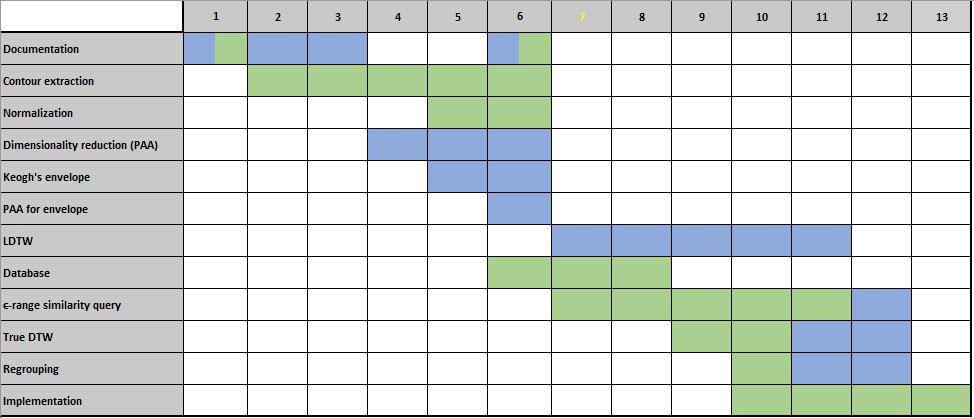
\includegraphics[width=10cm]{orga_prev.PNG}
	\end{center}
	\colorbox[HTML]{A9D08E}{\textcolor[HTML]{FFFFFF}{Florent}}
	\colorbox[HTML]{8ea9db}{\textcolor[HTML]{FFFFFF}{Arnaud}}
\end{frame}
\end{document}
